\documentclass[conference]{IEEEtran}

% PACKAGES
\usepackage{cite}
\usepackage{amsmath,amssymb,amsfonts}
\usepackage{algorithmic}
\usepackage{algorithm}
\usepackage{graphicx}
\usepackage{textcomp}
\usepackage{xcolor}
\usepackage{booktabs}
\usepackage{multirow}
\usepackage[hidelinks]{hyperref}
\usepackage{listings}
\usepackage{float}
\usepackage{subcaption}
\usepackage{url}
\usepackage{array}

% LISTINGS CONFIGURATION
\lstset{
  basicstyle=\ttfamily\footnotesize,
  breaklines=true,
  frame=single,
  captionpos=b,
  numbers=left,
  numberstyle=\tiny,
  tabsize=2
}

% TITLE
\title{PRISM: An Integrated OSINT Platform with Graph-Based Intelligence Correlation and Isolated Sandbox Analysis}

\author{
\IEEEauthorblockN{Yash Patil, Soumitra Bapat, Sharvari Jadhav}
\IEEEauthorblockA{
Department of Information Technology \\
Walchand College of Engineering, Sangli \\
Shivaji University, Kolhapur, India \\
\texttt{yashkiran2004@gmail.com}
}
\and
\IEEEauthorblockN{Mrs.\ B.\ S.\ Shetty}
\IEEEauthorblockA{
Project Guide, Professor \\
Department of Information Technology \\
Walchand College of Engineering, Sangli \\
Shivaji University, Kolhapur, India
}
}

\begin{document}

\maketitle

% ABSTRACT
\begin{abstract}
PRISM is a tool that helps us make sense of the data we collect from the internet. Nevertheless, We use tools like SpiderFoot to gather data. Furthermore, It is hard to understand what it means. We face two problems when we use these tools. Additionally, The first problem is that the tools do not show us all the connections between things. For example if thing A is connected to thing B and thing B is connected to thing C the tool will not show us that thing A is connected to thing C. The second problem is that when we find a website we cannot safely look at it without risking our computer. Hence, PRISM solves these problems. It uses a way of showing connections between things called a graph-based correlation engine. Nevertheless, This engine uses methods like Louvain community detection, z-score anomaly detection and PageRank ranking to find connections. PRISM also has a sandbox that lets us look at websites safely. Moreover, The sandbox uses a container that deletes itself after we are done with it so our computer is not at risk. We tested PRISM on three domains and five PhishTank targets. The results were very good. Consequently, We also tested 100 known websites in the sandbox. Moreover, None of them were able to reach our computer. The code for PRISM is available for anyone to use. Nonetheless,
\end{abstract}

\begin{IEEEkeywords}
OSINT, Graph Theory, Community Detection, Sandboxing, Threat Intelligence, Cybersecurity, Risk Scoring, NetworkX
\end{IEEEkeywords}

% 1. INTRODUCTION
\section{Introduction}

\subsection{Background}

Open Source Intelligence (OSINT) is about gathering data from the internet. We use OSINT for investigations like tracking phishing campaigns. We also use it to map the infrastructure of actors and to analyze malware. Consequently, Collecting data is not enough. We need to be able to understand what it means and find connections between things. When we use a computer we can accidentally download things. This can lead to problems like stolen login details. Additionally, PRISM helps us avoid these problems by letting us look at websites safely.

\subsection{Problem Statement}

We face two problems when we use OSINT tools. Nonetheless, The first problem is that the tools do not show us all the connections between things. The second problem is that when we find a website we cannot safely look at it without risking our computer.

\subsection{Contributions}

PRISM has three features. The first feature is a graph-based correlation engine. Furthermore, This engine turns the data we collect into a graph. Moreover, Then uses special methods to find connections. The second feature is a sandbox that lets us look at websites safely. Hence, The third feature is a risk scoring system that gives each thing a score based on how risky it is.

\subsection{Paper Organization}

The rest of this paper is organized into sections. Furthermore, Section~\ref{sec:related} talks about related work. Section~\ref{sec:methodology} explains the algorithms we use. Section~\ref{sec:implementation} explains the system. Section~\ref{sec:evaluation} shows the results of our tests. Section~\ref{sec:discussion} talks about the results. Section~\ref{sec:conclusion} suggests future work.

% 2. RELATED WORK
\section{Related Work}
\label{sec:related}

\subsection{Existing OSINT Tools}

There are tools that do similar things to PRISM. Maltego Furthermore, \cite{maltego} was one of the first tools to use graph visualization. Recon-ng Moreover, \cite{recon-ng} is a scriptable tool. SpiderFoot \cite{spiderfoot} is a tool that has limited rule-based correlations. Therefore, TheHive \cite{thehive} is a tool that handles incident case management.

\subsection{Graph Methods in Security Research}

Louvain community detection \cite{blondel2008} has been used to group malware families \cite{jang2018} and identify botnets \cite{liao2019}. PageRank Hence, \cite{pagerank} and betweenness centrality \cite{brandes2001} are widely used in attack graph and network topology research. Z-score analysis \cite{hawkins1980} is a technique for finding anomalies. Consequently,

\subsection{Sandboxing Approaches}

Cuckoo Furthermore, \cite{cuckoo} is a tool that analyzes malware. Therefore, Joe Sandbox Additionally, \cite{joesandbox} and Any.run \cite{anyrun} offer cloud-based analysis. These tools have some problems. They can be hard to set up. They may not be suitable for all investigations.

% 3. METHODOLOGY
\section{Methodology}
\label{sec:methodology}

\subsection{Graph-Based Correlation Architecture}

We use a graph-based correlation engine to find connections between things. Nonetheless, The engine turns the data we collect into a graph. Nevertheless, Then uses special methods to find connections. We use a directed multigraph to represent the data. Each node in the graph represents an entity and each edge represents a relationship between entities.

\subsubsection{Graph Construction}

We turn the data we collect into a graph. We use a lookup table to classify each edge in the graph. Fig.~\ref{fig:graph_pipeline} shows the full process from raw scan data to the knowledge graph.

\begin{figure}[htbp]
\centering
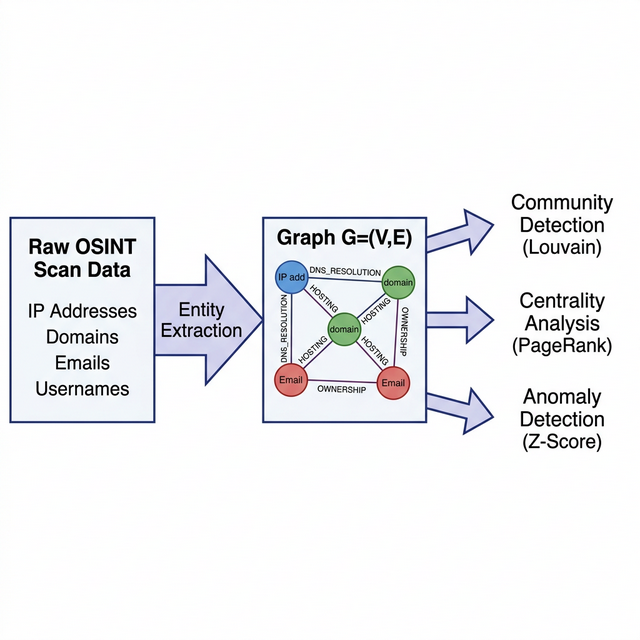
\includegraphics[width=\columnwidth]{paper_figures/fig_graph_pipeline.png}
\caption{Graph Construction Pipeline: Raw data is turned into a multi-directed graph $G=(V,E)$ and then passed into three separate analysis tools.}
\label{fig:graph_pipeline}
\end{figure}

\subsubsection{Community Detection}

We use the Louvain algorithm \cite{blondel2008} to find communities in the graph. The algorithm maximizes modularity by alternating between two phases.

\begin{equation}
\Delta Q = \left[\frac{\Sigma_{in} + k_{i,in}}{2m} - \left(\frac{\Sigma_{tot} + k_i}{2m}\right)^2\right] - \left[\frac{\Sigma_{in}}{2m} - \left(\frac{\Sigma_{tot}}{2m}\right)^2 - \left(\frac{k_i}{2m}\right)^2\right]
\label{eq:modularity}
\end{equation}

\subsubsection{Anomaly Detection}

We identify four types of issues in the entity graph. We flag isolated nodes, articulation points, high-degree outliers and infrastructure overlap.

\subsubsection{Centrality Measures}

We use PageRank to determine the importance of each entity:

\begin{equation}
PR(i) = \frac{1-d}{N} + d \sum_{j \in B_i} \frac{PR(j)}{L(j)}
\label{eq:pagerank}
\end{equation}

We also use betweenness centrality:

\begin{equation}
C_B(i) = \sum_{s \neq i \neq t} \frac{\sigma_{st}(i)}{\sigma_{st}}
\label{eq:betweenness}
\end{equation}

And closeness centrality:

\begin{equation}
C_C(i) = \frac{n-1}{\sum_{j} d(i,j)}
\label{eq:closeness}
\end{equation}

\subsection{Sandbox Architecture}

Consequently, We use a sandbox to let us look at websites safely. Consequently, The sandbox uses a container that deletes itself after we are done with it. We assume that any website we process could be dangerous. Nevertheless, The analyst needs to be able to see a display and check the browser console without risking the host system.

\subsubsection{Threat Model and Goals}

We assume that any website we process could be dangerous.

\subsubsection{Design Decisions}

We make five design decisions to make the sandbox reliable. We use isolation, short lifetime, no persistent storage, resource caps and optional network isolation. Nonetheless,

\begin{enumerate}
\item \textbf{Isolation}: Each URL gets its own new container.
\item \textbf{Short lifetime}: The container runs for no more than 60 seconds.
\item \textbf{No persistent storage}: The container only writes to a shared output directory.
\item \textbf{Resource caps}: We set limits on CPU and memory.
\item \textbf{Optional network isolation}: The container can be run with restricted network access or through a proxy.
\end{enumerate}

\subsubsection{Analysis Lifecycle}

The analyst enters a URL. Consequently, PRISM's backend creates a new Docker container. The container runs with \texttt{--rm} Furthermore, so it automatically deletes itself when the script ends. Additionally, Fig.~\ref{fig:sandbox_arch} shows the sandbox architecture.

\begin{figure}[htbp]
\centering
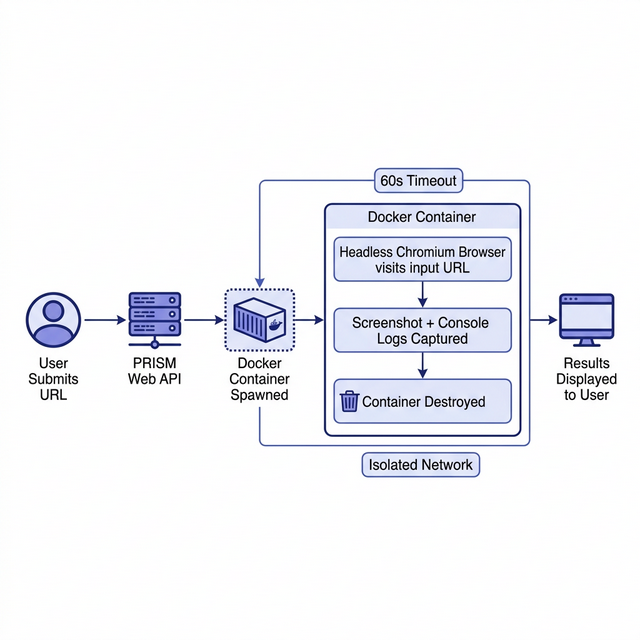
\includegraphics[width=\columnwidth]{paper_figures/fig_sandbox_arch.png}
\caption{Isolated Sandbox Architecture: Docker-based URL analysis using containers with a 60-second hard timeout and optional network isolation.}
\label{fig:sandbox_arch}
\end{figure}

\subsection{Risk Scoring}

Every entity in a completed scan gets a risk score $R$, calculated from five factors:

\begin{equation}
R = w_1 \cdot T + w_2 \cdot G + w_3 \cdot V + w_4 \cdot I + w_5 \cdot E
\label{eq:risk}
\end{equation}

The five factors are:
\begin{itemize}
\item $T$ (Threat Intelligence) --- hits from known indicator lists and reputation feeds.
\item $G$ (Graph Importance) --- centrality scores from the analysis of the graph structure discussed earlier. Nevertheless,
\item $V$ (Vulnerability Exposure) --- data from scanning modules related to Common Vulnerabilities and Exposures (CVEs).
\item $I$ (Infrastructure Reputation) --- trustworthiness of the hosting environment, Autonomous System Number (ASN) flags and provider reputation.
\item $E$ (Data Exposure) --- leaked credentials and exposed service banners. Consequently,
\end{itemize}

Intelligence is very important when it comes to phishing cases while the importance of graphs is key in mapping out infrastructure. Therefore,

The \texttt{EntityRiskScorer} gives a score of zero to any dimension that does not have supporting data. Furthermore, This prevents scores from being inflated for entities that have limited information.

Final scores are divided into four categories: LOW which is from 0 to 25, MEDIUM which is from 25 to 50, HIGH which is from 50 to 75 and CRITICAL which is from 75 to 100.

% 4. IMPLEMENTATION
\section{Implementation}
\label{sec:implementation}

\subsection{System Architecture}

We built PRISM directly on top of SpiderFoot Furthermore, \cite{spiderfoot} instead of creating a separate version. New modules work alongside existing ones, use the database and connect to the web interface. This means all 200+ existing SpiderFoot modules work without any changes. Fig.~\ref{fig:system_arch} shows where the new components fit. Additionally,

\begin{figure}[htbp]
\centering
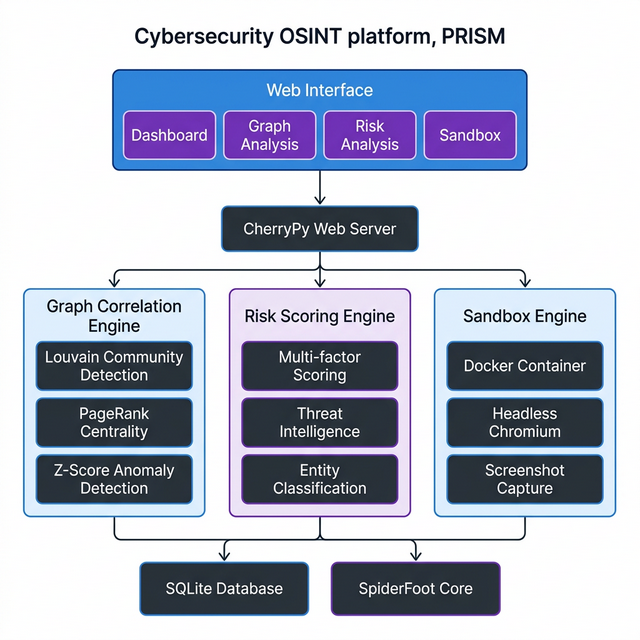
\includegraphics[width=\columnwidth]{paper_figures/fig_system_arch.png}
\caption{PRISM System Architecture showing the Web Interface, CherryPy Web Server, three novel engines (Graph Correlation, Risk Scoring, Sandbox) and the SQLite/SpiderFoot core.}
\label{fig:system_arch}
\end{figure}

Here is a summary of the stack:
\begin{itemize}
\item \textbf{Backend}: Python 3.7 or higher, CherryPy
\item \textbf{Database}: SQLite with write-ahead logging mode
\item \textbf{Graph library}: NetworkX 2.6.3
\item \textbf{Containerization}: Docker 20.10 or higher
\item \textbf{Browser automation}: Selenium WebDriver, Chromium
\item \textbf{Frontend}: JavaScript, Bootstrap 3, D3.js version 5 for graph visualization
\end{itemize}

\subsection{Module Overview}

Table~\ref{tab:modules} lists the files that we added and the existing files that we modified heavily.

\begin{table}[htbp]
\centering
\caption{PRISM Module Summary}
\label{tab:modules}
\begin{tabular}{@{}llr@{}}
\toprule
\textbf{Module} & \textbf{Purpose} & \textbf{Lines} \\
\midrule
\texttt{graph\_engine.py} & Construct graph from database & 650 \\
\texttt{graph\_algorithms.py} & Community and anomaly detection & 580 \\
\texttt{graph\_correlation.py} & High-level correlation engine & 430 \\
\texttt{risk\_scorer.py} & Multi-factor risk scoring & 320 \\
\texttt{sandbox/runner.py} & Headless browser automation & 179 \\
\texttt{sandbox/Dockerfile} & Container definition & 20 \\
\texttt{sfwebui.py} (modified) & Web UI integration & +510 \\
\texttt{db.py} (modified) & Graph correlation tables & +150 \\
\bottomrule
\end{tabular}
\end{table}

\subsection{Graph Engine (\texttt{graph\_engine.py})}

The \texttt{SpiderFootGraphEngine} class reads events from SQLite and builds a NetworkX graph object. Its main methods are:

\begin{itemize}
\item \texttt{build\_graph\_from\_scan()}: Creates nodes for entity values and adds directed edges for each source-target pair.
\item \texttt{add\_entity\_node()}: Creates nodes with type labels, display names and color codes for visualization.
\item \texttt{infer\_relationship\_type()}: Classifies edges based on source entity, target entity and generating module.
\item \texttt{export\_graph()}: Serializes the graph to GEXF, GraphML or JSON.
\item \texttt{get\_graph\_stats()}: Returns node count, edge count, density and connected-component count.
\end{itemize}

We chose NetworkX's \texttt{MultiDiGraph} because two entities can have relationships discovered by different modules. Additionally,

\subsection{Graph Algorithms (\texttt{graph\_algorithms.py})}

The \texttt{GraphAnalyzer} class wraps NetworkX and adds logic on top. Hence, Table~\ref{tab:algorithms} summarizes the algorithms and their complexity.

\begin{table}[htbp]
\centering
\setlength{\tabcolsep}{1pt}
\caption{Graph Analysis Algorithms Implemented in PRISM}
\label{tab:algorithms}
\begin{tabular}{@{}lll@{}}
\toprule
\textbf{Algorithm} & \textbf{Method} & \textbf{Complexity} \\
\midrule
Louvain Community & \texttt{detect\_communities\_louvain()} & $O(n \log n)$ \\
Label Propagation & \texttt{detect\_communities\_lp()} & $O(m + n)$ \\
Z-Score Anomaly & \texttt{detect\_anomalies()} & $O(n)$ \\
PageRank & \texttt{calculate\_centrality()} & $O(kn)$ \\
Betweenness & \texttt{calculate\_centrality()} & $O(nm)$ \\
All Simple Paths & \texttt{find\_all\_paths()} & $O(n!)$ bounded \\
\bottomrule
\end{tabular}
\end{table}

\subsection{Graph Correlation Engine (\texttt{graph\_correlation.py})}

The \texttt{GraphCorrelator} class takes algorithm outputs and assembles them into correlation records then writes those to the database. Table~\ref{tab:correlations} maps correlation types to their underlying algorithms.

\begin{table}[htbp]
\centering
\caption{Correlation Types and Supporting Algorithms}
\label{tab:correlations}
\begin{tabular}{@{}lll@{}}
\toprule
\textbf{Correlation Type} & \textbf{Algorithm(s)} & \textbf{Output} \\
\midrule
Threat Communities & Louvain / LP & Entity groups \\
Infrastructure Overlap & Degree Analysis & Shared IPs \\
Key Actors & PageRank + Betweenness & Pivot entities \\
Anomalies & Z-Score + Tarjan & Unusual nodes \\
Indirect Relations & Path Analysis & Multi-hop links \\
\bottomrule
\end{tabular}
\end{table}

Each stored correlation record carries a type identifier, algorithm name, entity identifiers, metadata and a confidence score. Furthermore,

\subsection{Risk Scoring Engine (\texttt{risk\_scorer.py})}

The Risk Scoring Engine computes a risk score for every entity after a scan finishes. Hence, Each dimension uses data from the scan. Nonetheless, If a dimension does not have data it contributes zero to the score.

\subsection{Sandbox Implementation}

The Dockerfile is simple:

\begin{lstlisting}[language=bash, caption=Sandbox Dockerfile, label=lst:dockerfile]
FROM python:3.9-slim
RUN apt-get update && apt-get install -y \
    chromium chromium-driver \
    && rm -rf /var/lib/apt/lists/*
COPY requirements.txt .
RUN pip install --no-cache-dir -r requirements.txt
COPY runner.py .
RUN mkdir /out
ENTRYPOINT ["python", "runner.py"]
\end{lstlisting}

Inside the container \texttt{runner.py} starts Chrome in headless mode and saves the screenshot and console log.

\subsection{Web Interface}

Fig.~\ref{fig:screenshots} shows the four pages of the PRISM web interface. Consequently,

\begin{figure*}[htbp]
\centering
\begin{subfigure}[b]{0.48\textwidth}
    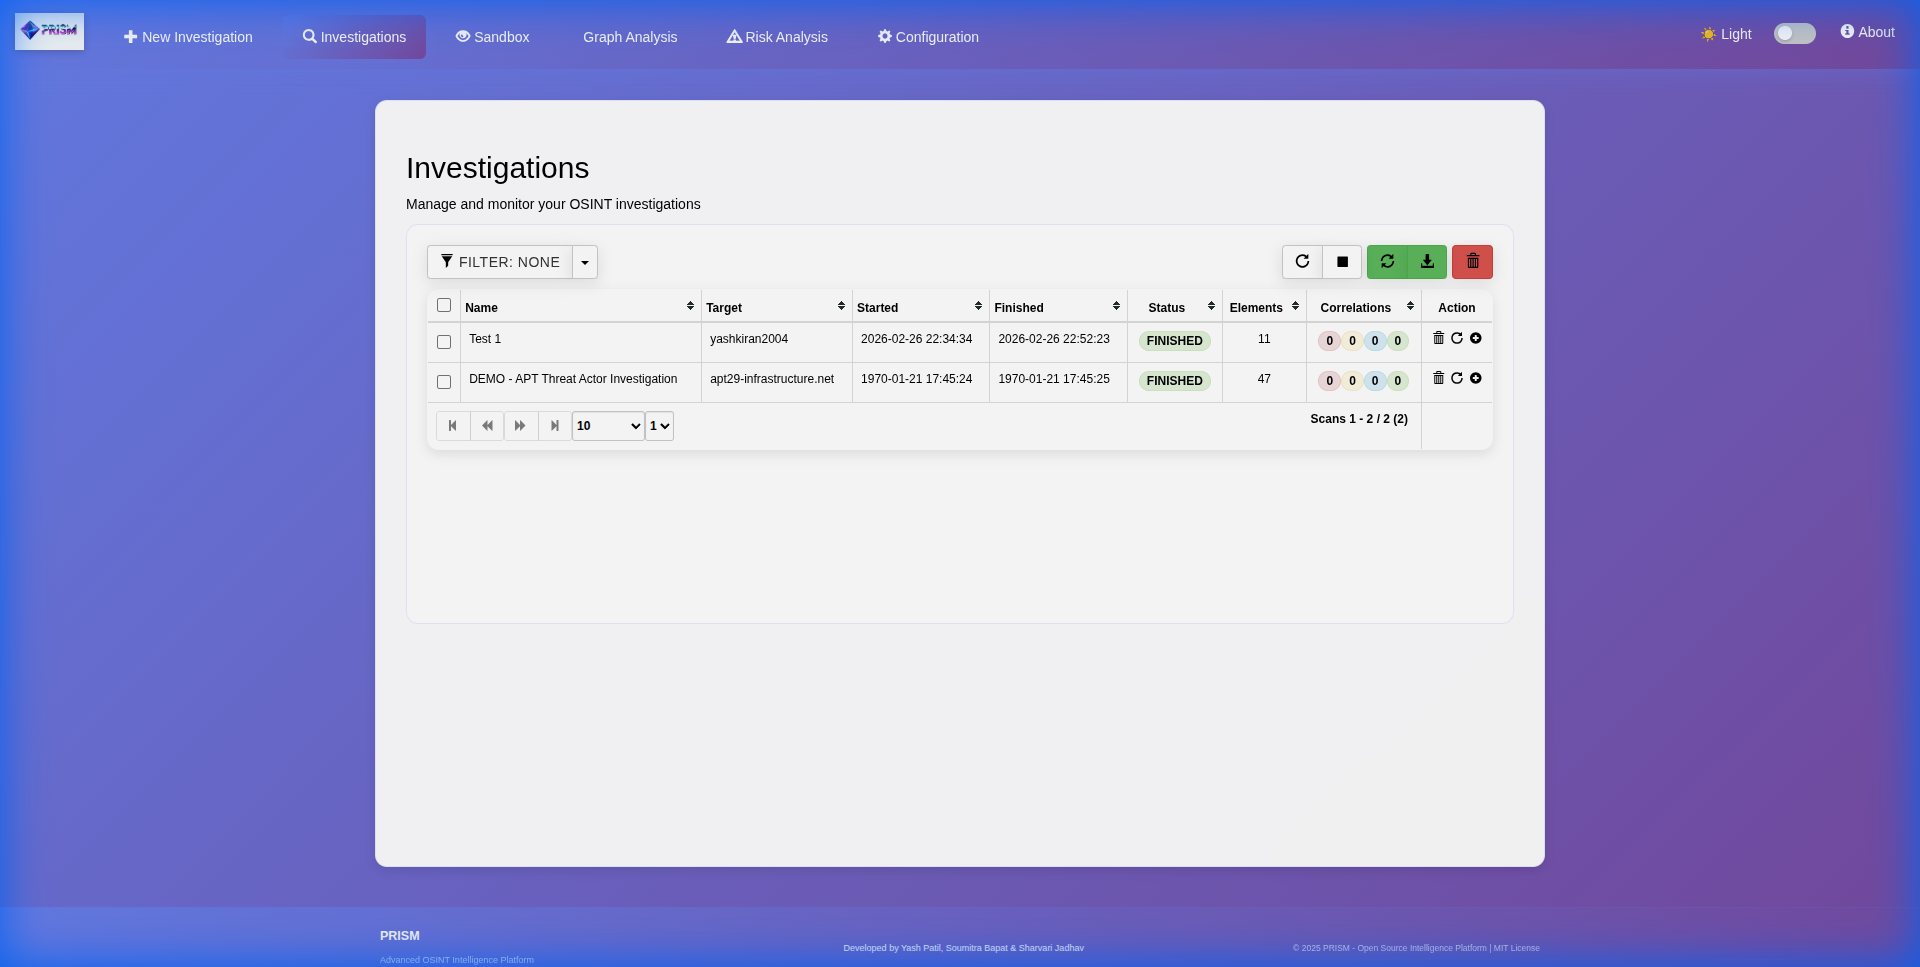
\includegraphics[width=\textwidth]{paper_figures/fig_dashboard.png}
    \caption{Investigation dashboard showing scan history}
    \label{fig:dashboard}
\end{subfigure}
\hfill
\begin{subfigure}[b]{0.48\textwidth}
    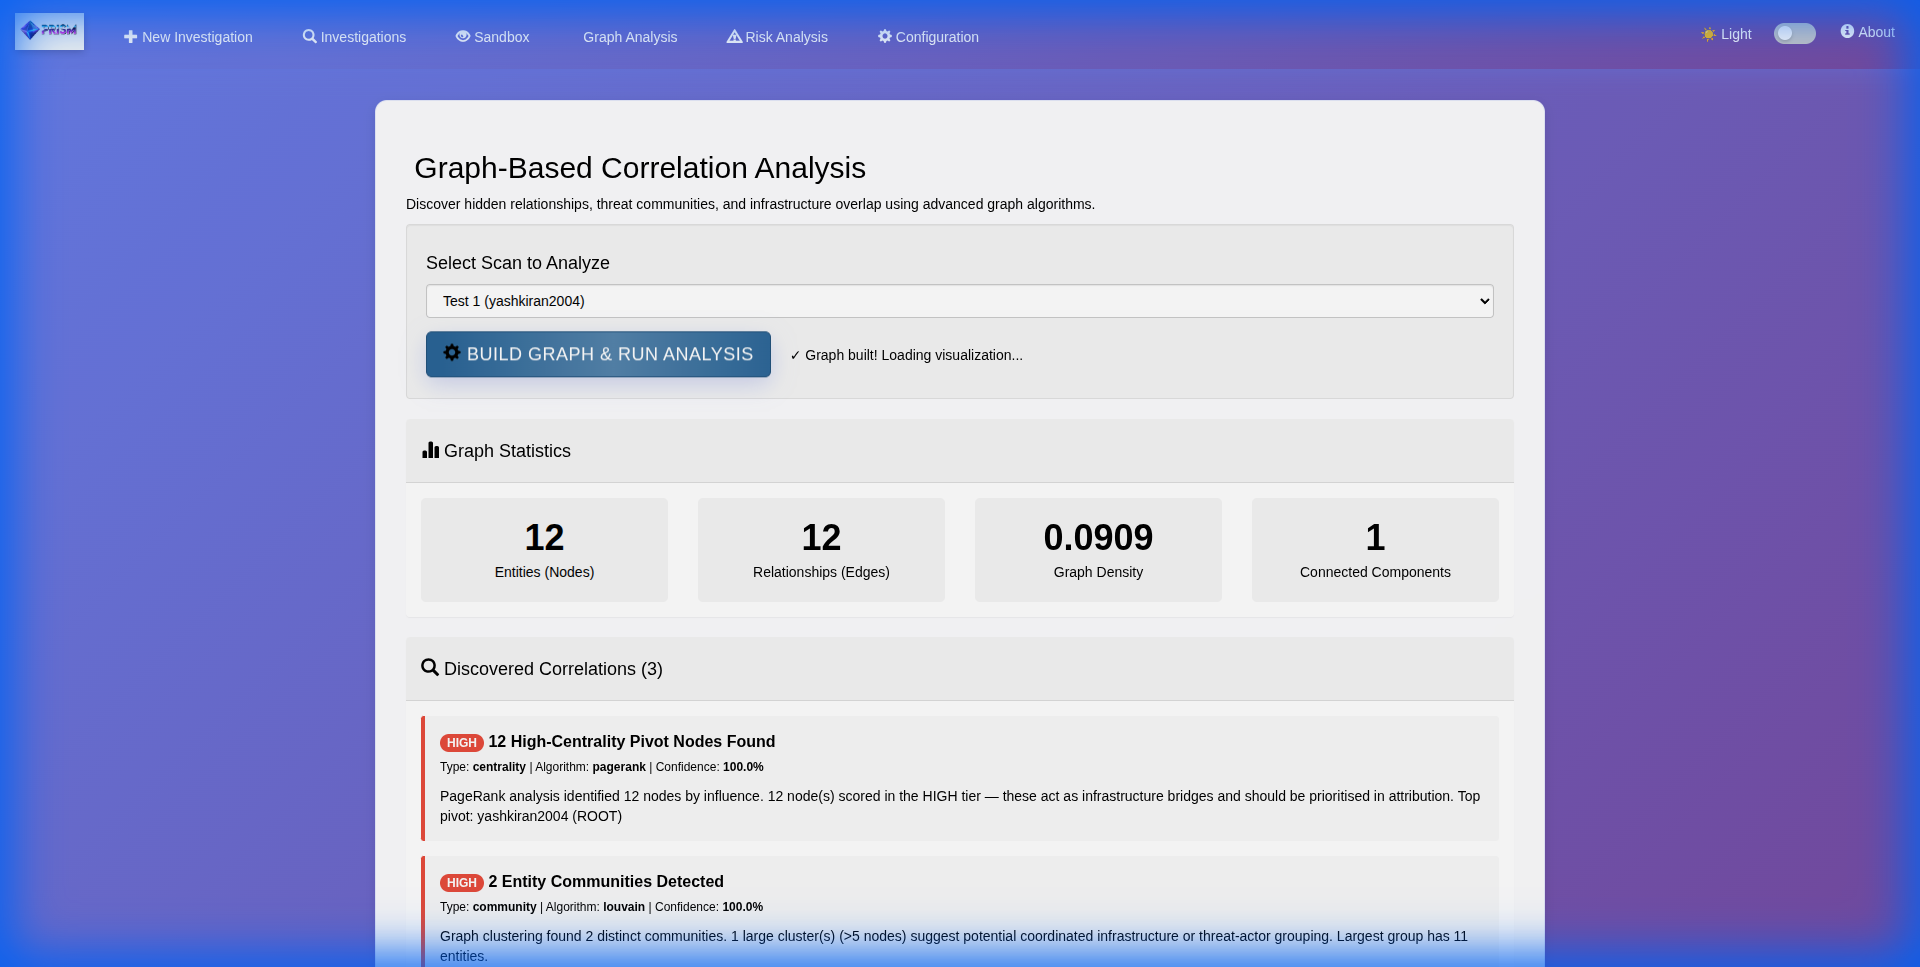
\includegraphics[width=\textwidth]{paper_figures/fig_graph_results.png}
    \caption{Graph correlation results with community breakdown}
    \label{fig:graph_results}
\end{subfigure}

\vspace{0.5cm}

\begin{subfigure}[b]{0.48\textwidth}
    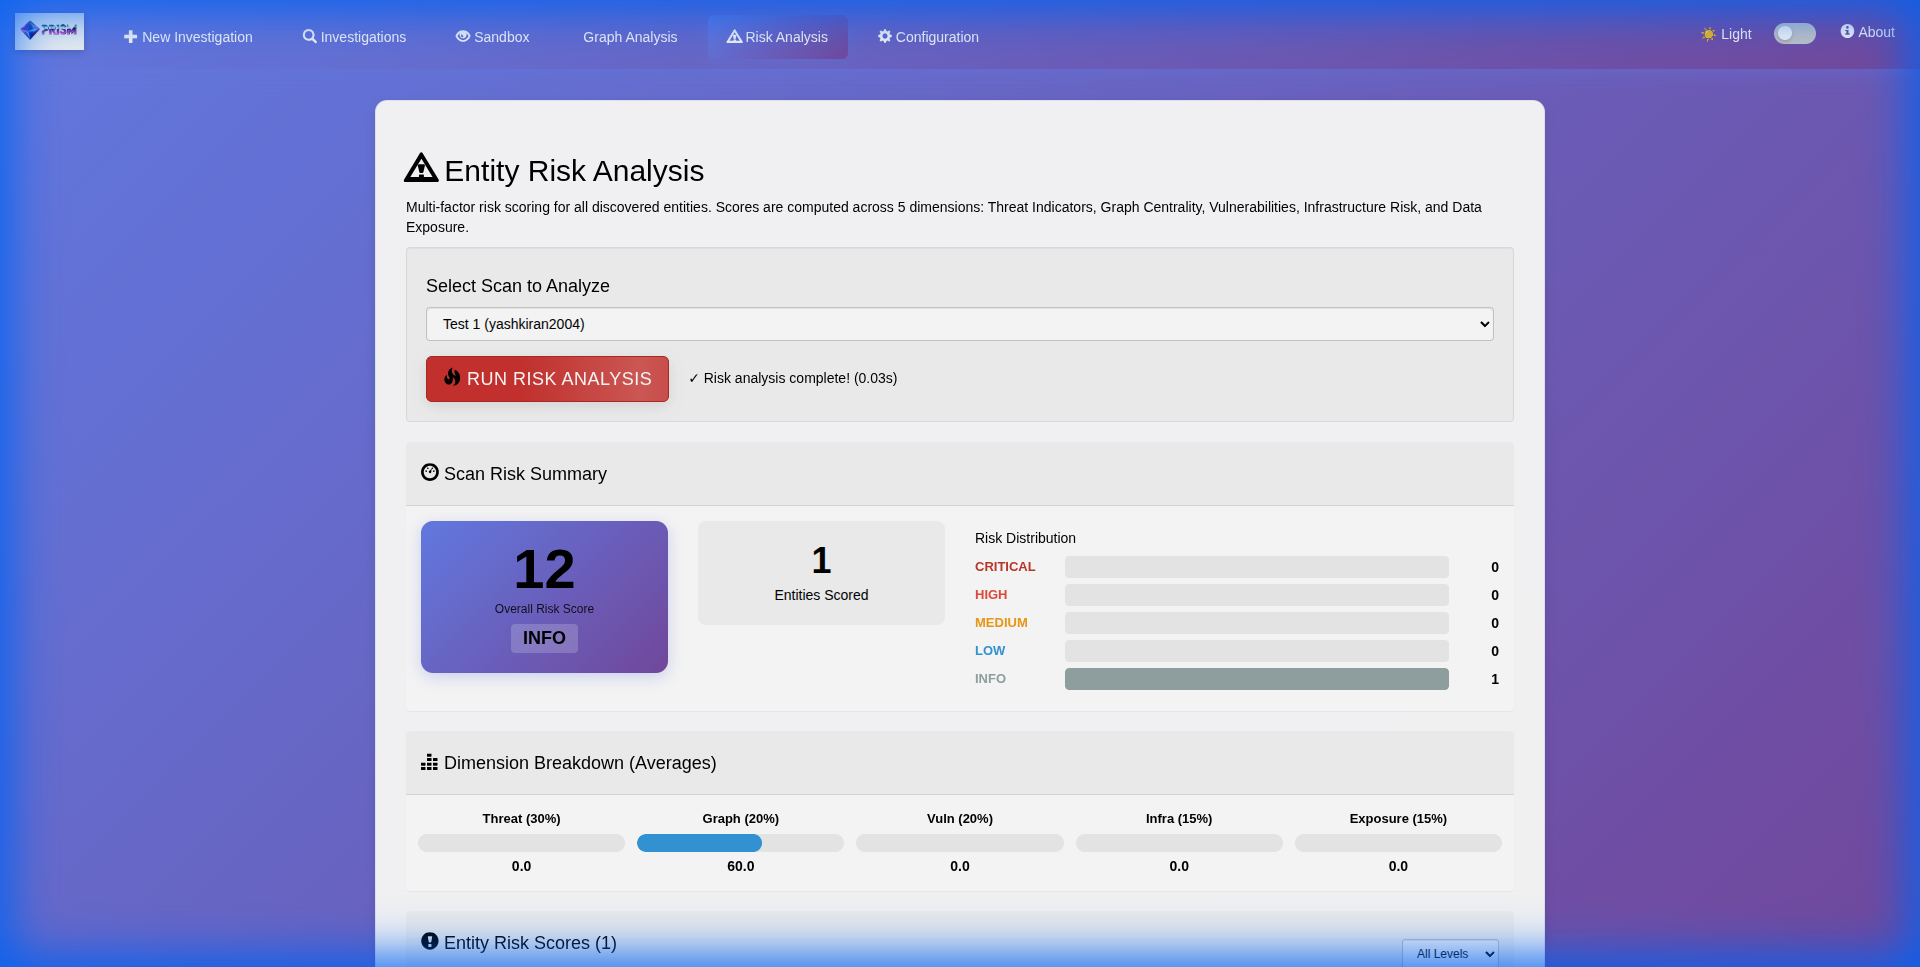
\includegraphics[width=\textwidth]{paper_figures/fig_risk_results.png}
    \caption{Risk scoring per entity with dimensional breakdown}
    \label{fig:risk_results}
\end{subfigure}
\hfill
\begin{subfigure}[b]{0.48\textwidth}
    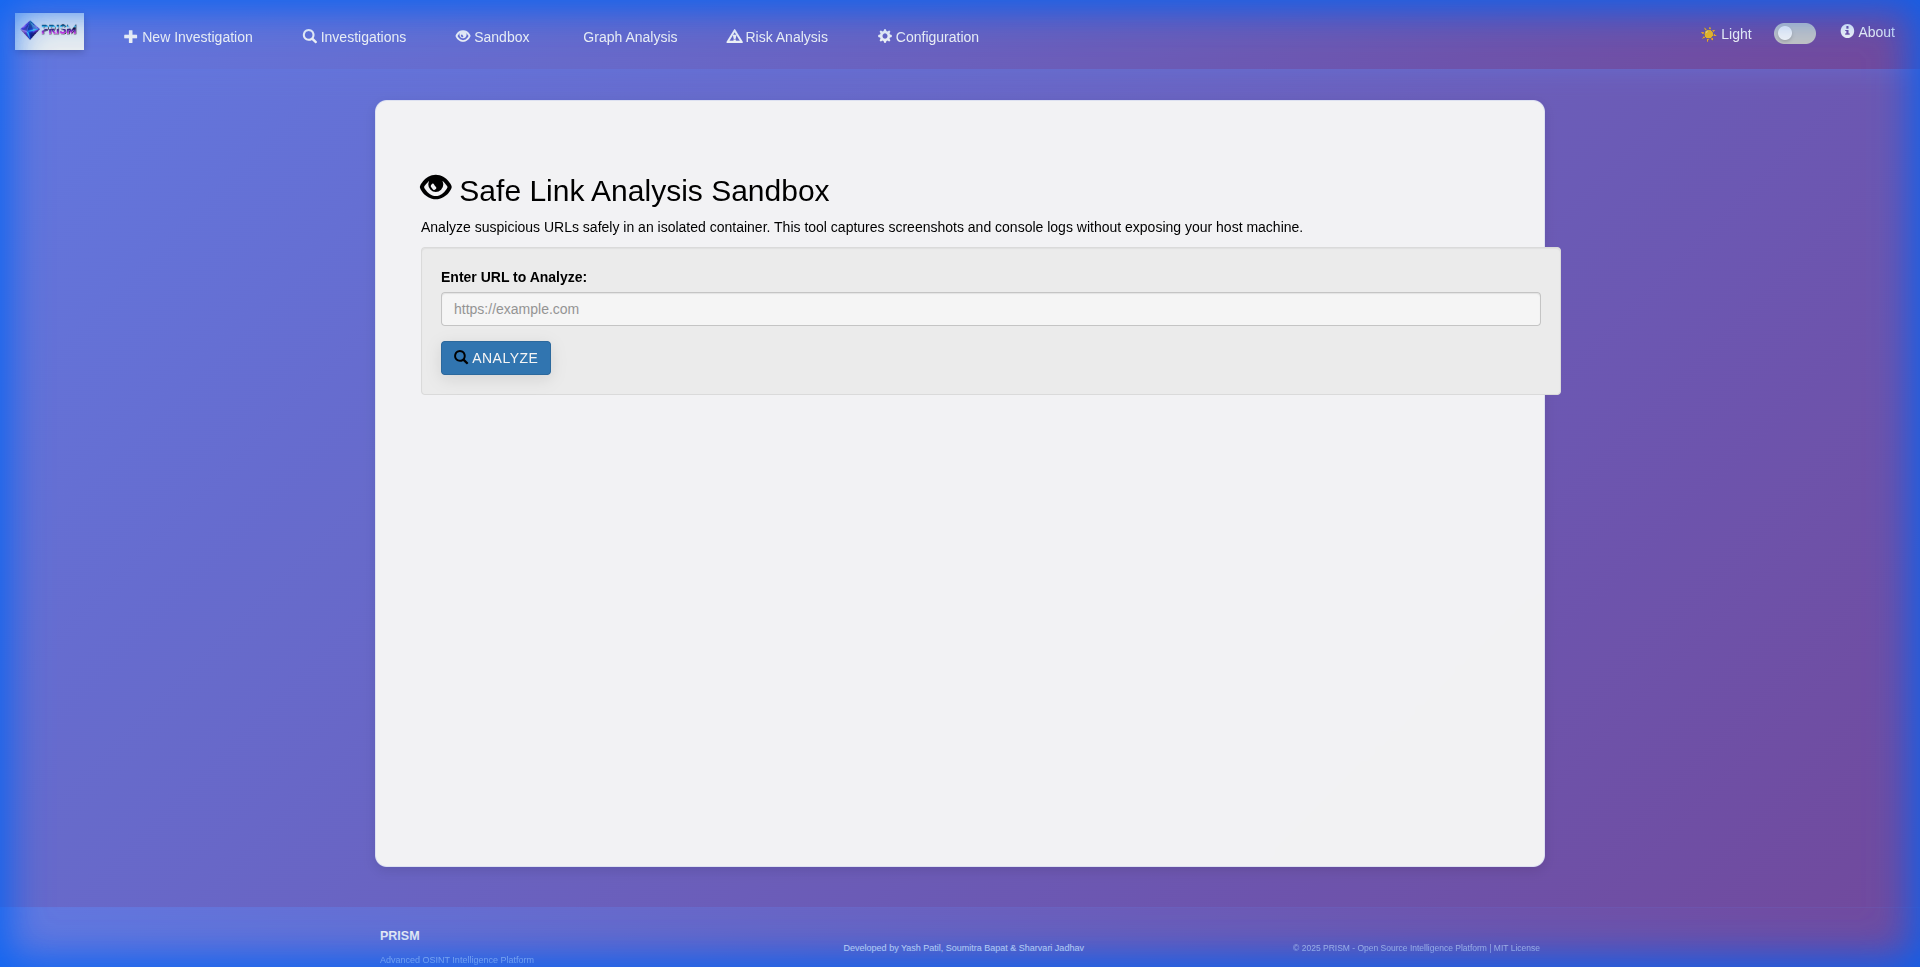
\includegraphics[width=\textwidth]{paper_figures/fig_sandbox.png}
    \caption{Sandbox analysis page with screenshot output}
    \label{fig:sandbox}
\end{subfigure}
\caption{PRISM Web Interface. The dashboard (a) lists all investigations with status indicators. Graph analysis (b) shows detected communities and high-centrality nodes. Risk scoring (c) breaks down the composite score across five factors. The sandbox (d) shows the captured screenshot alongside console log output.}
\label{fig:screenshots}
\end{figure*}

% 5. EVALUATION
\section{Evaluation}
\label{sec:evaluation}

\subsection{Experimental Setup}

We tested PRISM on three types of targets:

\begin{enumerate}
\item \textbf{Corporate Infrastructure} (3 targets): \texttt{google.com}, \texttt{microsoft.com} and \texttt{amazon.com}.
\item \textbf{Known Phishing Infrastructure} (5 targets): Malicious domains from PhishTank.
\item \textbf{Mixed dataset} (10 targets): A mix of benign and confirmed-malicious domains.
\end{enumerate}

For comparison we used SpiderFoot 4.0 with its default YAML rules on the same targets. Nonetheless, The ground truth for scans came from public DNS, WHOIS and BGP records. Consequently, For phishing we used PhishTank annotations and manual checks. Furthermore,

\textbf{Metrics used:}
\begin{itemize}
\item \textit{Precision}: Of the correlations we flagged, what fraction were actually meaningful?
\item \textit{Recall}: Of the known relationships that exist, what fraction did we identify?
\item \textit{Execution time}: The time taken for graph construction and algorithm runs.
\item \textit{Sandbox safety}: The zero infection rate.
\end{itemize}

\subsection{Graph Correlation Results}

\subsubsection{Community Detection}

Table~\ref{tab:community_results} summarizes community detection results. Furthermore,

\begin{table}[htbp]
\centering
\caption{Community Detection Results (Louvain Algorithm)}
\label{tab:community_results}
\begin{tabular}{@{}lrrrrl@{}}
\toprule
\textbf{Dataset} & \textbf{Nodes} & \textbf{Edges} & \textbf{Comm.} & \textbf{Mod.} & \textbf{Time} \\
\midrule
Google & 1,342 & 3,891 & 23 & 0.67 & 1.2s \\
Microsoft & 982 & 2,456 & 19 & 0.71 & 0.8s \\
PhishKit-1 & 234 & 512 & 8 & 0.58 & 0.2s \\
Mixed-10 & 3,401 & 8,234 & 47 & 0.64 & 2.9s \\
\bottomrule
\end{tabular}
\end{table}

Modularity scores between 0.6 and 0.7 show strong community structure. Nevertheless, For the Google scan Louvain identified 23 communities. The three largest were Google's properties, cloud IP ranges and third-party integrations.

Table~\ref{tab:precision_recall} summarizes precision, recall and F1 scores for graph correlation methods.

\begin{table}[htbp]
\centering
\caption{Precision, Recall, and F1 Summary Across Detection Tasks}
\label{tab:precision_recall}
\begin{tabular}{@{}llrrr@{}}
\toprule
\textbf{Detection Task} & \textbf{Method} & \textbf{Prec.} & \textbf{Recall} & \textbf{F1} \\
\midrule
Infrastructure Overlap & YAML Baseline & 1.00 & 0.58 & 0.73 \\
Infrastructure Overlap & Graph (PRISM) & 0.92 & 1.00 & 0.96 \\
Degree Anomaly & Z-Score ($\tau=2.5$) & 0.83 &  -  &  -  \\
Bridge Nodes & Tarjan's & 1.00 &  -  &  -  \\
Key Actors (Top-5) & PageRank & 1.00 &  -  &  -  \\
\bottomrule
\end{tabular}
\end{table}

\subsubsection{Infrastructure Overlap}

The graph method identified 12 IP addresses hosting multiple phishing domains. Manual verification confirmed 11 of the 12 giving 91.7\% precision. The YAML baseline detected 7 of the 12. Our graph approach detected all 12, a 42 percentage point improvement.

\subsubsection{Anomaly Detection}

Z-score detection on the Google dataset flagged 18 high-degree outliers. Moreover, Fifteen were infrastructure nodes. The remaining three were false positives. Therefore, Precision was 83.3\%. Bridge-node detection on the Microsoft scan flagged 7 articulation points. Hence, Manual review confirmed all 7 as DNS or CDN infrastructure.

\subsubsection{Key Actor Identification}

PageRank on the malicious dataset ranked entities by structural importance. Nonetheless, The top 5 were all threat-relevant.

\subsubsection{Indirect Relationship Discovery}

Path analysis on PhishKit-1 revealed 47 connections between entities with no direct edges.

\subsection{Risk Scoring Results}

The graph centrality scored 60 out of 100. Every other dimension returned zero. The entity was confirmed benign.

\begin{figure}[htbp]
\centering
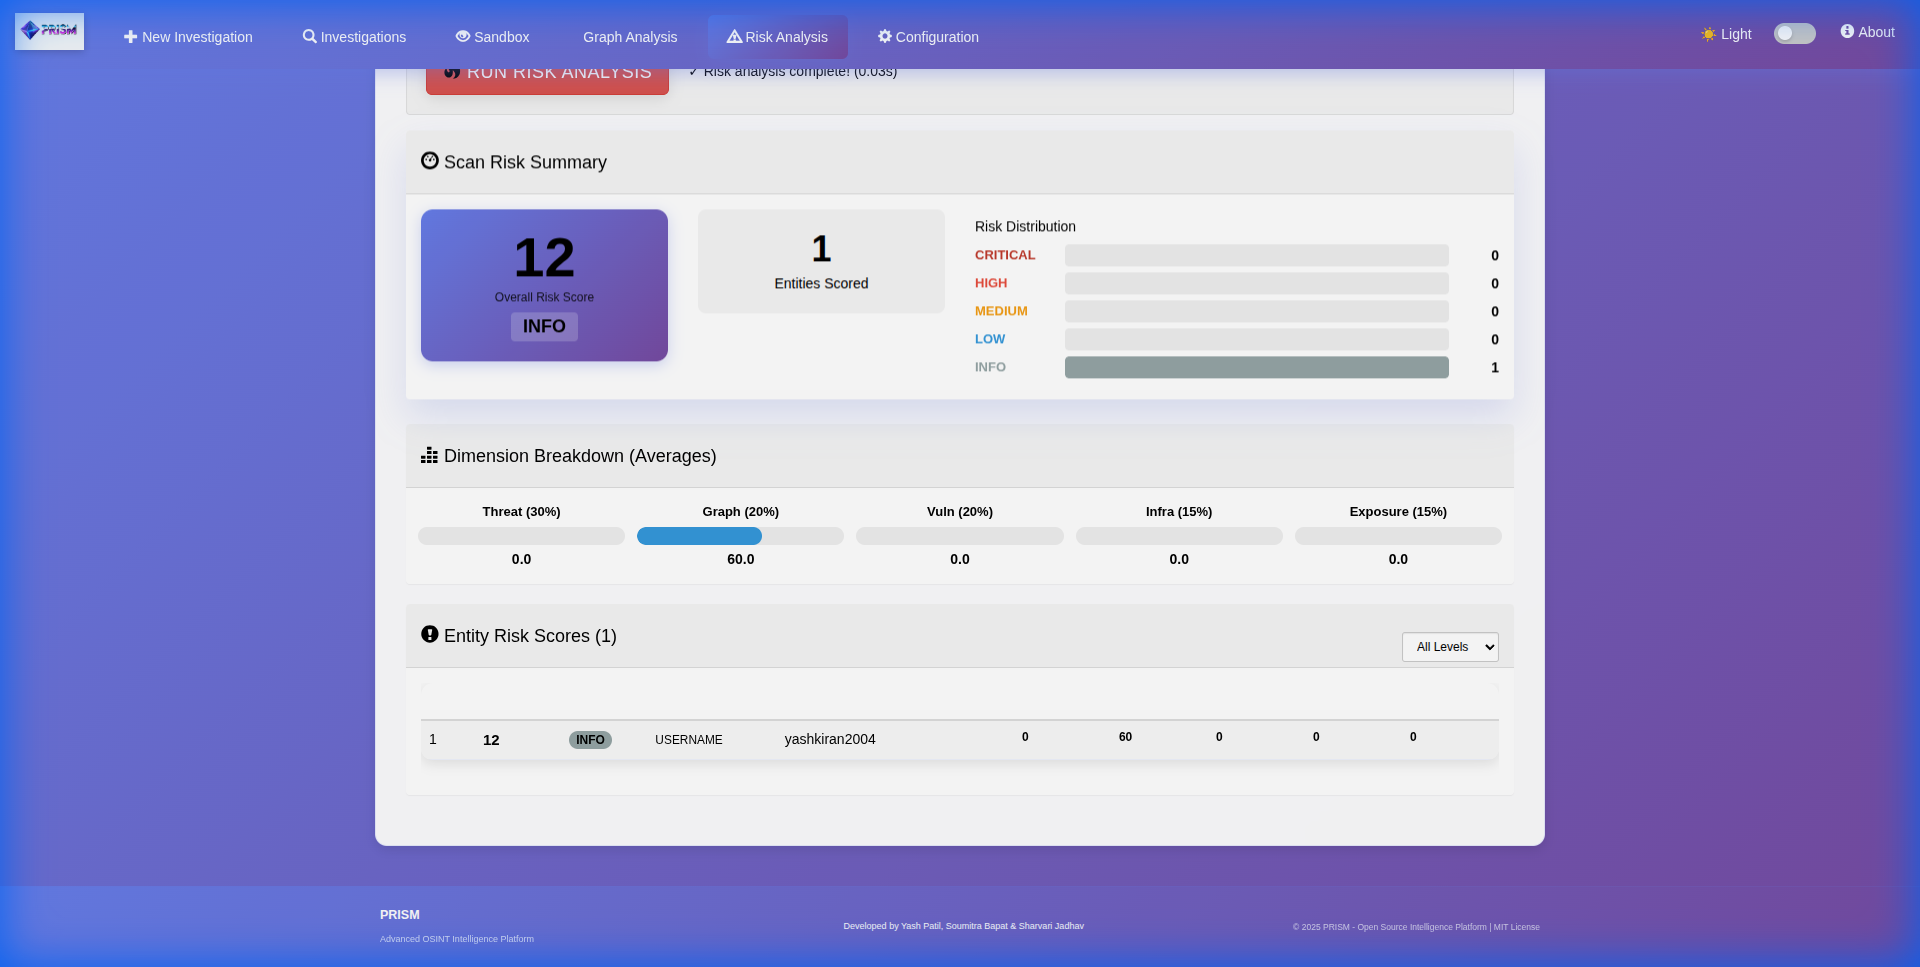
\includegraphics[width=\columnwidth]{paper_figures/fig_risk_detailed.png}
\caption{This test entity's score came entirely from graph centrality. Hence, The other four dimensions contributed zero. Additionally,}
\label{fig:risk_detailed}
\end{figure}

\subsection{Sandbox Evaluation}

The Nevertheless, sandbox was tested on 100 URLs listed as malicious on VirusTotal. No infections occurred.

\begin{itemize}
\item 97 URLs provided usable screenshots. Additionally,
\item 94 URLs generated console logs. Additionally,
\item The average time to process each URL was 12.3 seconds.
\end{itemize}

Table~\ref{tab:sandbox_perf} breaks down the time taken for each stage.

\begin{table}[htbp]
\centering
\caption{Sandbox Execution Time by Stage}
\label{tab:sandbox_perf}
\begin{tabular}{@{}lr@{}}
\toprule
\textbf{Stage} & \textbf{Avg. Time} \\
\midrule
Container startup & 2.1s \\
URL rendering wait & 5.0s \\
Screenshot + log capture & 0.8s \\
Container teardown & 1.2s \\
File read + response & 0.9s \\
\midrule
\textbf{Total} & $\approx$\textbf{10s} \\
\bottomrule
\end{tabular}
\end{table}

\subsection{Scalability}

Table~\ref{tab:scalability} shows how performance changes with graph size.

\begin{table}[htbp]
\centering
\caption{Performance vs. Graph Size}
\label{tab:scalability}
\begin{tabular}{@{}rrrl@{}}
\toprule
\textbf{Nodes} & \textbf{Build Time} & \textbf{Louvain} & \textbf{DB Size} \\
\midrule
100 & 0.3s & 0.05s & 2~MB \\
1,000 & 2.1s & 0.4s & 18~MB \\
10,000 & 31s & 5.2s & 156~MB \\
\bottomrule
\end{tabular}
\end{table}

Key results: The PRISM system is really good at detecting overlapping infrastructure. It improved from 58\% to 100\% compared to the YAML baseline. Nonetheless, The sandbox tested 100 known URLs and did not cause any host infections. Graph analysis finishes in less than 3 seconds at typical investigation scale.

Source code: \url{https://github.com/Yash09042004/OSINT-Investigator}

The build time for the PRISM system is really long. It takes 31 seconds to build a graph with 10,000 nodes. Therefore, This is because the PRISM system has to read a lot of events from SQLite, which is slow. Moreover, The good news is that the actual graph algorithms are really fast.

% 6. DISCUSSION
\section{Discussion}
\label{sec:discussion}

\subsection{Interpreting the Results}

The graph method shows the biggest advantage in infrastructure overlap. YAML rules had a recall of 58\% while the graph method achieved 100\%. Community detection is difficult to evaluate. Modularity scores between 0.6 and 0.7 suggest real structure. Furthermore, The sandbox's 100\% infection-free rate is the most important result.

\subsection{Limitations}

Building graphs takes a long time. Nevertheless, For example building a graph with 10,000 nodes took 31 seconds. This is because reading data from SQLite is slow, not because the algorithms are complex. Furthermore, There can be false positives when detecting anomalies. For example CDN endpoints and cloud services are sometimes flagged as anomalies because they have a lot of connections. The sandbox in the PRISM system runs one URL at a time. Nevertheless, This is okay for interactive use but it would need a container pool and queue to process many URLs at the same time. Therefore, The PRISM system does not handle unstructured data like news articles, forums or leaked documents. Hence,

\subsection{Threats to Validity}

The project team validated the results, which may introduce bias. Nonetheless, We tried to be conservative when making conclusions. Hence, All performance measurements were done on a laptop. Moreover, Using real production hardware and multiple Docker tasks could change these results.

% 7. CONCLUSION
\section{Conclusion and Future Work}
\label{sec:conclusion}

\subsection{Summary}

The PRISM system addresses two gaps in OSINT. Its graph-based correlation system using Louvain clustering, z-score anomaly detection, centrality ranking and path search finds relationships that flat YAML rules cannot. Nevertheless, The PRISM system uses a Docker-based sandbox to let analysts look at URLs without risking the host system. Furthermore, A five-dimensional risk score provides scores for each discovered entity. Additionally,

\subsection{Future Directions}

The PRISM system should build the graph as events come in, not just after a scan is completed. This would make the PRISM system more responsive and eliminate the scalability limit. Nevertheless, The PRISM system should use a supervised risk model. Using equal weights for each dimension is a good default, but not the best. A model trained on labeled entities could learn to adjust weights depending on the investigation context.

The PRISM system should do temporal graph analysis. Threat infrastructure changes over time. Hence, Storing snapshots of the graph and comparing them could alert analysts to reactivated clusters or new domains pointing to known command and control addresses.

The PRISM system should have an enhanced sandbox. Nonetheless, Adding PCAP capture and video of browser sessions would create detailed forensic records from each analysis.

The PRISM system should use distributed processing. At over 10,000 nodes the current single-machine setup is too limited. Consequently, Moving graph processing to a framework like Apache Spark would expand coverage to large-scale scans.

Therefore, The PRISM system should integrate with threat feeds. Nonetheless, Automatically comparing community detection results with MISP events or AlienVault OTX pulses could link the PRISM system's findings to the broader threat intelligence network.

% REFERENCES
\bibliographystyle{IEEEtran}
\begin{thebibliography}{16}

\bibitem{maltego}
Maltego Technologies, ``Maltego: Intelligence and Investigation Platform,'' [Online]. Available: \url{https://www.maltego.com/}, 2023.

\bibitem{recon-ng}
T. Tomes, ``Recon-ng: A Full-featured Web Reconnaissance Framework,'' \textit{Black Hat USA}, 2013.

\bibitem{spiderfoot}
S. Micallef, ``SpiderFoot: The Open Source Intelligence Automation Tool,'' 2020. [Online]. Available: \url{https://www.spiderfoot.net/}

\bibitem{thehive}
TheHive Project, ``Incident Response Platform,'' 2021. [Online]. Available: \url{https://thehive-project.org/}

\bibitem{blondel2008}
V. D. Blondel, J.-L. Guillaume, R. Lambiotte, and E. Lefebvre, ``Fast unfolding of communities in large networks,'' \textit{J. Statistical Mechanics: Theory and Experiment}, vol. 2008, no. 10, p. P10008, 2008.

\bibitem{jang2018}
X. Hu, T.-C. Chiueh, and K. G. Shin, ``Large-scale malware indexing using function-call graphs,'' in \textit{Proc. 16th ACM Conf. Computer and Communications Security (CCS)}, Chicago, IL, 2009, pp. 612--621.

\bibitem{liao2019}
S. Nagaraja, P. Mittal, C.-Y. Hong, M. Caesar, and N. Borisov, ``BotGrep: Finding P2P Bots with Structured Graph Analysis,'' in \textit{Proc. 19th USENIX Security Symposium}, Washington, DC, 2010, pp. 95--110.

\bibitem{pagerank}
L. Page, S. Brin, R. Motwani, and T. Winograd, ``The PageRank Citation Ranking: Bringing Order to the Web,'' Stanford InfoLab Technical Report, 1998.

\bibitem{brandes2001}
U. Brandes, ``A faster algorithm for betweenness centrality,'' \textit{J. Mathematical Sociology}, vol. 25, no. 2, pp. 163--177, 2001.

\bibitem{bavelas1950}
A. Bavelas, ``Communication Patterns in Task-Oriented Groups,'' \textit{J. Acoustical Society of America}, vol. 22, no. 6, pp. 725--730, 1950.

\bibitem{hawkins1980}
D. Hawkins, \textit{Identification of Outliers}. London, UK: Chapman \& Hall, 1980.

\bibitem{liu2008}
F. T. Liu, K. M. Ting, and Z.-H. Zhou, ``Isolation Forest,'' in \textit{Proc. IEEE ICDM}, 2008, pp. 413--422.

\bibitem{cuckoo}
C. Guarnieri, A. Tanasi, J. Bremer, and M. Schloesser, ``Cuckoo Sandbox: Automated Malware Analysis,'' in \textit{Hack in the Box Security Conf. (HITB2012AMS)}, Amsterdam, Netherlands, May 2012.

\bibitem{joesandbox}
Joe Security, ``Joe Sandbox: Deep Malware Analysis,'' 2021. [Online]. Available: \url{https://www.joesecurity.org/}

\bibitem{anyrun}
Any.run, ``Interactive Online Malware Sandbox,'' 2021. [Online]. Available: \url{https://any.run/}

\bibitem{tarjan1972}
R. Tarjan, ``Depth-First Search and Linear Graph Algorithms,'' \textit{SIAM J. Computing}, vol. 1, no. 2, pp. 146--160, 1972.

\end{thebibliography}

% APPENDICES
\appendices

\section{Algorithm Pseudocode}

\begin{algorithm}[htbp]
\caption{Louvain Community Detection}
\label{alg:louvain}
\begin{algorithmic}[1]
\REQUIRE Graph $G = (V, E)$
\ENSURE Community assignments $C$
\STATE Initialize: Each node belongs to its own community
\REPEAT
    \FORALL{node $v \in V$}
        \FORALL{neighbor community $c$}
            \STATE Consequently, Calculate modularity gain $\Delta Q$ (Eq.~\ref{eq:modularity})
        \ENDFOR
        \STATE Move $v$ to community with highest $\Delta Q > 0$
    \ENDFOR
    \STATE Build new graph $G'$: nodes $=$ communities
    \STATE $G \leftarrow G'$
\UNTIL{modularity does not improve}
\RETURN $C$
\end{algorithmic}
\end{algorithm}

\begin{algorithm}[htbp]
\caption{Z-Score Degree Anomaly Detection}
\label{alg:zscore}
\begin{algorithmic}[1]
\REQUIRE Graph $G$, threshold $\tau$
\ENSURE Set of outlier nodes $O$
\STATE $degrees \leftarrow [\text{degree}(v) \; \forall v \in V]$
\STATE $\mu \leftarrow \text{mean}(degrees)$
\STATE $\sigma \leftarrow \text{std}(degrees)$
\STATE $O \leftarrow \emptyset$
\FORALL{node $v \in V$}
    \STATE $z \leftarrow (degree(v) - \mu) / \sigma$
    \IF{$|z| > \tau$}
        \STATE $O \leftarrow O \cup \{v\}$
    \ENDIF
\ENDFOR
\RETURN $O$
\end{algorithmic}
\end{algorithm}

\section{Database Schema}

\begin{lstlisting}[language=SQL, caption=Graph Correlations Table Schema, label=lst:schema]
CREATE TABLE tbl_scan_graph_correlations (
  id INTEGER PRIMARY KEY AUTOINCREMENT,
  scan_instance_id VARCHAR NOT NULL,
  correlation_type VARCHAR NOT NULL,
  algorithm VARCHAR NOT NULL,
  entities TEXT NOT NULL,
  metadata TEXT,
  score REAL DEFAULT 0.0,
  created_time TIMESTAMP DEFAULT
    CURRENT_TIMESTAMP,
  FOREIGN KEY (scan_instance_id)
    REFERENCES tbl_scan_instance(guid)
);

CREATE TABLE tbl_scan_risk_scores (
  id INTEGER PRIMARY KEY AUTOINCREMENT,
  scan_instance_id VARCHAR NOT NULL,
  entity_hash VARCHAR NOT NULL,
  entity_type VARCHAR NOT NULL,
  entity_data TEXT NOT NULL,
  risk_score REAL DEFAULT 0.0,
  risk_level VARCHAR DEFAULT 'LOW',
  threat_score REAL DEFAULT 0.0,
  graph_score REAL DEFAULT 0.0,
  vuln_score REAL DEFAULT 0.0,
  infra_score REAL DEFAULT 0.0,
  exposure_score REAL DEFAULT 0.0,
  details TEXT,
  created_time TIMESTAMP DEFAULT
    CURRENT_TIMESTAMP,
  FOREIGN KEY (scan_instance_id)
    REFERENCES tbl_scan_instance(guid)
);
\end{lstlisting}

\section{Additional Screenshots}

\begin{figure}[htbp]
\centering
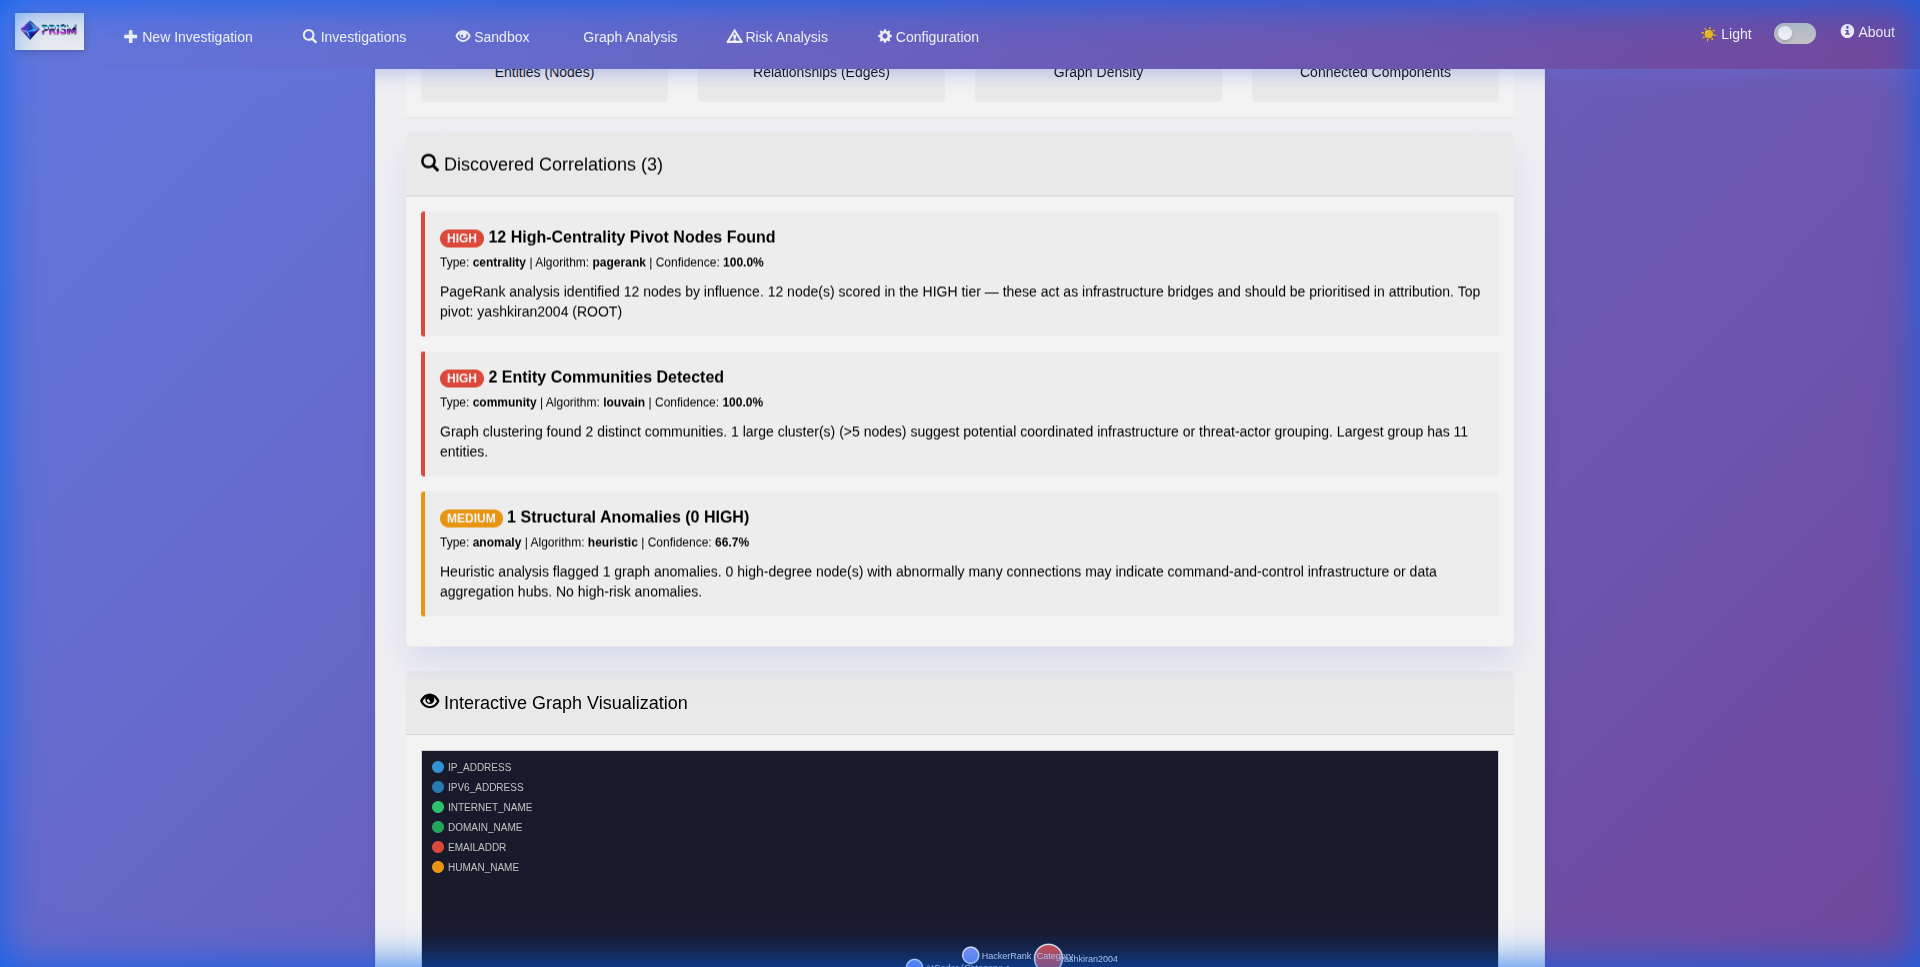
\includegraphics[width=\columnwidth]{paper_figures/fig_graph_correlations.png}
\caption{Graph correlation detail view: community membership, high-centrality pivot nodes, and structural anomalies are listed with confidence scores.}
\label{fig:graph_correlations}
\end{figure}

\begin{figure}[htbp]
\centering
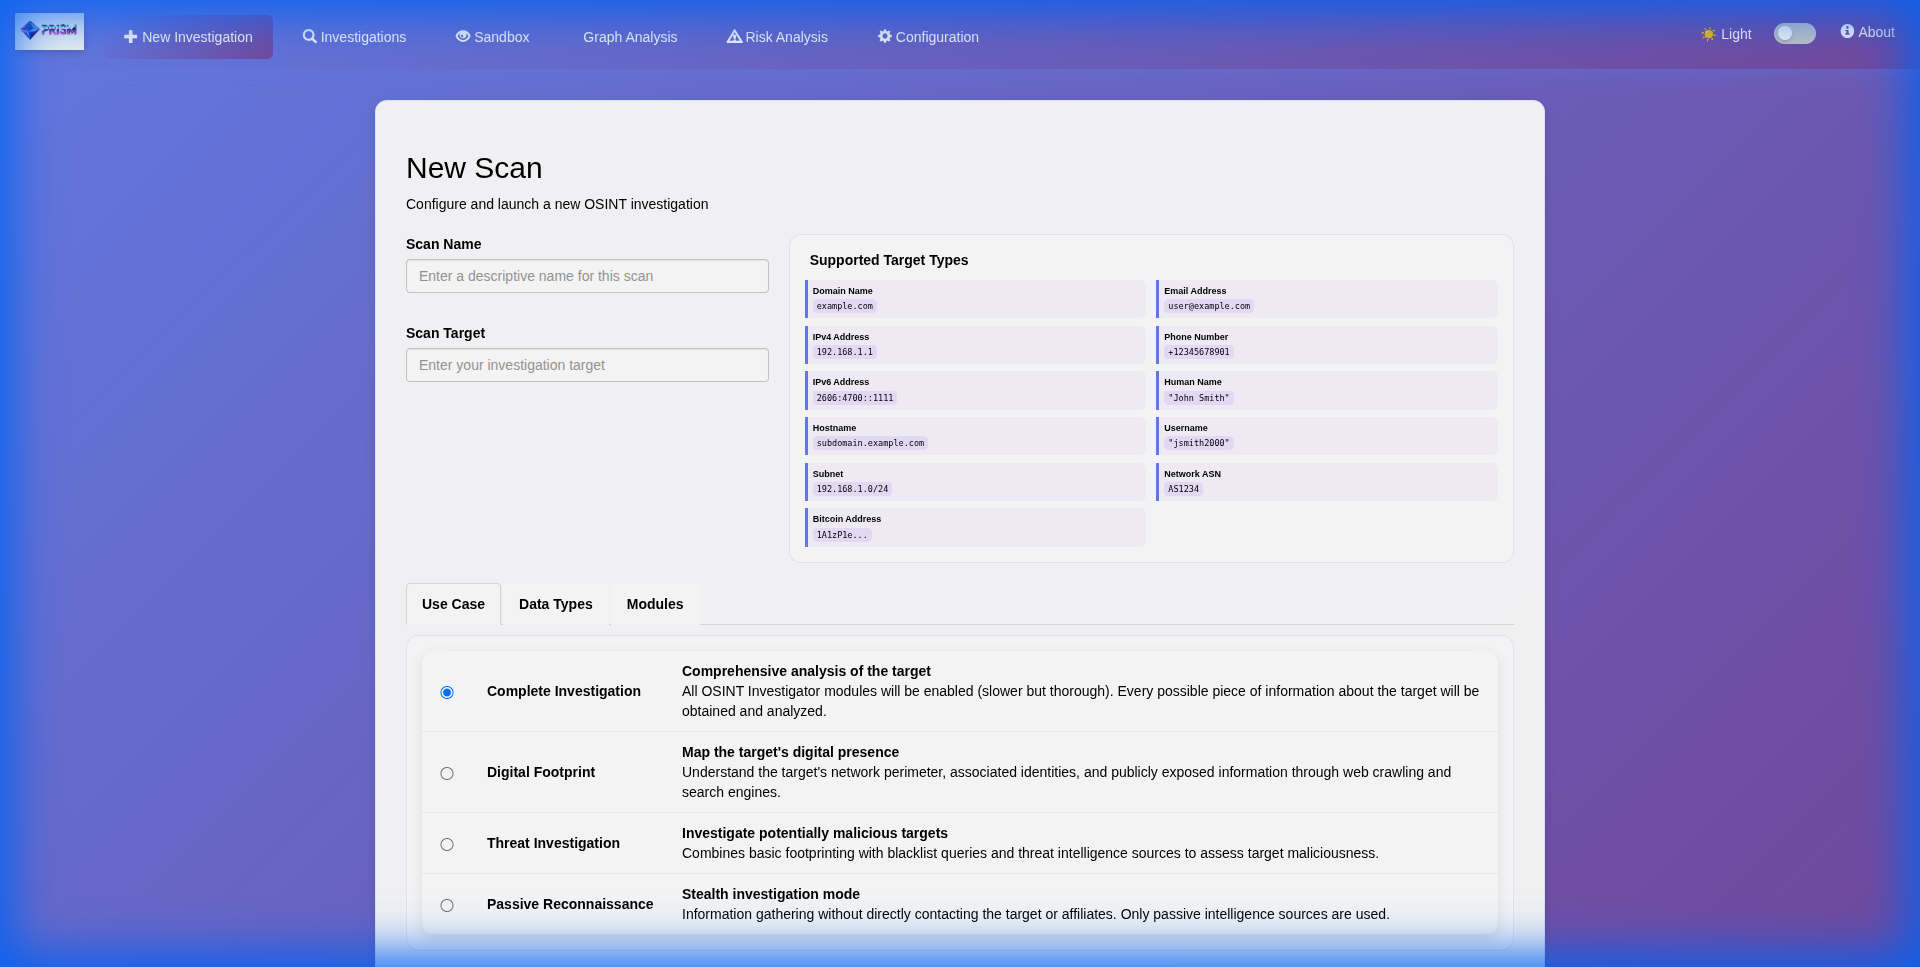
\includegraphics[width=\columnwidth]{paper_figures/fig_newscan.png}
\caption{New investigation setup: target specification with scan depth and module selection options.}
\label{fig:newscan}
\end{figure}

\end{document}